\documentclass[14pt, a4paper, titlepage, fleqn]{extarticle}

\usepackage{style/style}
\usepackage{style/titlepage}

\everymath{\displaystyle}

\begin{document}

    \fefutitlepage{
    ОТЧЁТ
}{
    к лабораторной работе №1 по дисциплине\\ <<Математическое и копмьютерное моделирование>>
}{
    01.03.02 <<Прикладная математика и информатика>>
}{
    Б9121-01.03.02сп
}{
    Держапольский Ю.В.
}{
    Профессор к.ф.-м. н.
}{
    Пермяков М. С.
}
    
    \tableofcontents

    \pagebreak

    \section{Введение}
    Во нашем мире большое количество явлений это колебания, например, звук -- это колебания воздуха, свет -- колебания электромагнитных волн. И математический маятник -- это фундаментальная модель идеальных колебаний. В отличие от физического маятника, мы не учитываем внешние факторы и представляем маятник наиболее просто -- как материальную точку, движущуюся в одной плоскости. Однако, также представляет интерес и взаимодействие каких-либо внешних сил на маятник.
    
    \pagebreak
    
    \section{Модель Лотки-Вольтерры}

    \subsection{Математическая модель}
    Классическая модель хищник-жертва для одной популяции жертвы \(x(t)\) и хищника \(y(t)\) называется такая модель\cite{svilog}:
    \begin{equation}
        \left\{\begin{split}
            & \dot{x} = \alpha(x) - V(x)y, \\
            & \dot{y} = k V(x)y -\beta(y),
        \end{split}\right. \label{lv-s}
    \end{equation}
    где коэффициенты \( \alpha, \beta \) -- функции естественного прироста жертв и естественной смертности хищников соответственно. Также их можно называть коэффициентом, обозначающим разность рождаемости и смертности в популяциях. Без взаимодеиствия жертвы беспрепятственно питаются и поэтому их рождается больше чем умирает, а у хищников -- из-за отсутствия питания -- наоборот, умирают больше, чем рождаются.

    Функция \( V(x) \) показывает количество жертв, потребляемых одним хищником за единицу времени, причём \(k\)-тая часть полученной с этой биомассой энергией расходуется хищником на воспроизводство. 
    
    При малых значениях \(x\), когда почти все жертвы становятся добычей хищника, который всегда голоден и насыщения не наступает, тогда функцию \( V(x) \) можно считать линейной функцией численности жертв: \( V = vx \). Беря функции прироста линейными, получим систему:
    \begin{equation}
        \left\{\begin{split}
            & \dot{x} = \alpha x - v x y, \\
            & \dot{y} = k v x y - \beta y,
        \end{split}\right. \label{lv-sl}
    \end{equation}
    Эта линейная система \eqref{lv-sl} совпадает с моделью В. Вольтерра, который показал, что такая система имеет неасимптотическую точку равновесия (центр) и поэтому эти популяции живут на замкнутых кривых на фазовой плоскости\cite{svilog}.

    Аналогичными предположениями приведём исследуемую схему (Рис. \ref{scheme}) к подобной системе:   
    \begin{equation}
        \left\{\begin{split}
            & \dot{x_1} = \varepsilon_1(x_1) - V_{12}(x_1)x_2 - V_{13}(x_1)x_3, \\
            & \dot{x_2} = \varepsilon_2(x_2) + k_{12} V_{12}(x_1)x_2 - V_{23}(x_2)x_3, \\
            & \dot{x_3} = -\varepsilon_3(x_3) + k_{13} V_{13}(x_1)x_3 + k_{23} V_{23}(x_2)x_3,
        \end{split}\right. \label{lv-g}
    \end{equation}
    где:
    \begin{enumerate}
        \item \( \varepsilon_i(x_i) \) -- функции прироста соответствующих популяций без взаимодействия с другими. Предполагаем, что жертва и первый хищник \(( x_1, x_2) \) имеют положительный прирост, а второй хищник \(( x_3 )\) -- отрицательный.
        \item \( V_{ij} (x_i) \) -- функции, показывающие какое количество из популяции \(x_i\) поглощается одним хищником популяции \( x_j \) за единицу времени. \(k_{ij}\) -- соответствующие части полученной при поглощении энергии, которые идут на воспроизводство популяции \(x_j\).
    \end{enumerate}
 
    Имеем автономную систему \( \dot{x} = f(x) \), где \( k_{ij} > 0 \). Аналогично примем функции в системе \eqref{lv-g} за линейные функции: 
    \[ \varepsilon_i(x_j) = \varepsilon_i \cdot x_j, ~ V_{ij}(x_k) = \alpha_{ij} \cdot x_k, \quad \varepsilon_i, \alpha_{ij} > 0 \]

    Тогда получим систему:
    \begin{equation}
        \left\{\begin{split}
            & \dot{x_1} = \varepsilon_1 x_1 - \alpha_{12} x_1 x_2 - \alpha_{13} x_1 x_3, \\
            & \dot{x_2} = \varepsilon_2 x_2 + k_{12} \alpha_{12} x_1 x_2 - \alpha_{23} x_2 x_3, \\
            & \dot{x_3} = -\varepsilon_3 x_3 + k_{13} \alpha_{13} x_1 x_3 + k_{23} \alpha_{23} x_2 x_3. 
        \end{split}\right. \label{lv-gl}
    \end{equation}

    Проанализируем, какое поведение популяций будет в этой модели.

    \pagebreak

    \subsection{Анализ модели}
    Матрица Якоби для данной системы:
    \[
        J = \frac{\partial f}{\partial x} = \left(\begin{matrix}
            \varepsilon_1 - \alpha_{12} x_2 - \alpha_{13} x_3 & -\alpha_{12} x_1 & -\alpha_{13} x_1 \\
            k_{12} \alpha_{12} x_2 & \varepsilon_2 + k_{12} \alpha_{12} x_1 - \alpha_{23} x_3 & -\alpha_{23} x_2 \\
            k_{13} \alpha_{13} x_3 & k_{23} \alpha_{23} x_3  & -\varepsilon_3 + k_{13} \alpha_{13} x_1 + k_{23} \alpha_{23} x_2
        \end{matrix}\right)
    \]

    Найдём точки равновесия дифференциального уравнения, т.е. решения \( (x_1, x_2, x_3) \) системы уравнений:
    \[
        \left\{\begin{split}
            & \varepsilon_1 x_1 - \alpha_{12} x_1 x_2 - \alpha_{13} x_1 x_3 = 0, \\
            & \varepsilon_2 x_2 + k_{12} \alpha_{12} x_1 x_2 - \alpha_{23} x_2 x_3 = 0, \\
            & -\varepsilon_3 x_3 + k_{13} \alpha_{13} x_1 x_3 + k_{23} \alpha_{23} x_2 x_3 = 0. 
        \end{split}\right.
        \Rightarrow
        \left\{\begin{split}
            & x_1 (\varepsilon_1 - \alpha_{12} x_2 - \alpha_{13} x_3) = 0, \\
            & x_2 (\varepsilon_2 + k_{12} \alpha_{12} x_1 - \alpha_{23} x_3) = 0, \\
            & x_3 (-\varepsilon_3 + k_{13} \alpha_{13} x_1 + k_{23} \alpha_{23} x_2) = 0. 
        \end{split}\right.
    \]

    \begin{enumerate}
        \item Если две любых переменных равны нулю, то в оставшейся строчке остаётся уравнение \( \varepsilon_i x_i = 0, \) т.е. все переменные равны нулю. Получаем тривиальное решение \( x^{(0)} = (0,0,0) \).
        \[
            J \big|_{x^{(0)}} = \left(\begin{matrix}
                \varepsilon_1 & 0 & 0 \\
                0 & \varepsilon_2 & 0 \\
                0 & 0  & -\varepsilon_3
            \end{matrix}\right)
        \]

        Откуда получаем собственные значения матрицы: 
        \[
            \lambda_1 = \varepsilon_1 > 0, \quad \lambda_2 = \varepsilon_2 > 0, \quad \lambda_1 = -\varepsilon_3 < 0.
        \]
        Значит около начала координат в плоскостях \( x_1 = 0, x_2 = 0 \) эта точка является седлом, а в \( x_3 = 0 \) -- неустойчивым узлом.
        \item Если \( x_1 = 0; x_2, x_3 \neq 0 \):
            \[
                \left\{\begin{split}
                    & \varepsilon_2 - \alpha_{23} x_3 = 0, \\
                    & -\varepsilon_3 + k_{23} \alpha_{23} x_2 = 0. 
                \end{split}\right.
                \Rightarrow
                x^{(1)} = \left( 0,\, \frac{\varepsilon_3}{k_{23} \alpha_{23}},\, \frac{\varepsilon_2}{\alpha_{23}} \right)
            \]

            \[
                A = J \big|_{x^{(1)}} = \left(\begin{matrix}
                    \varepsilon_1 - \alpha_{12} \frac{\varepsilon_3}{k_{23} \alpha_{23}} - \alpha_{13} \frac{\varepsilon_2}{\alpha_{23}} & 0 & 0 \\[10pt]
                    k_{12} \alpha_{12} \frac{\varepsilon_3}{k_{23} \alpha_{23}} & 0 & -\alpha_{23} \frac{\varepsilon_3}{k_{23} \alpha_{23}} \\[10pt]
                    k_{13} \alpha_{13} \frac{\varepsilon_2}{\alpha_{23}} & k_{23} \alpha_{23} \frac{\varepsilon_2}{\alpha_{23}}  & 0
                \end{matrix}\right)
            \]
            \[
                \det(\lambda I - A) = \left(\lambda - \left(\varepsilon_1 - \frac{\varepsilon_3 \alpha_{12} }{k_{23} \alpha_{23}} - \frac{\varepsilon_2 \alpha_{13}}{\alpha_{23}} \right) \right)(\lambda^2 + \varepsilon_2 \varepsilon_3) = 0.
            \]
            \[
                \lambda_1 = \varepsilon_1 - \frac{\varepsilon_3 \alpha_{12} }{k_{23} \alpha_{23}} - \frac{\varepsilon_2 \alpha_{13}}{\alpha_{23}} , \quad \lambda_{2,3} = \pm i \sqrt{\varepsilon_2 \varepsilon_3}.
            \]
            Точка \( x^{(1)} \) -- неустойчивая. В плоскости \( x_1 = 0 \) точка будет являться центром (асимптотически неустойчивая точка), т.е. создавать вокруг себя замкнутые кривые.

        \item Если \( x_2 = 0; x_1, x_3 \neq 0 \):
            \[
                \left\{\begin{split}
                    & \varepsilon_1 - \alpha_{13} x_3 = 0, \\
                    & -\varepsilon_3 + k_{13} \alpha_{13} x_1 = 0. 
                \end{split}\right.
                \Rightarrow
                x^{(2)} = \left( \frac{\varepsilon_3}{k_{13} \alpha_{13}},\, 0,\, \frac{\varepsilon_1}{\alpha_{13}} \right)
            \]

            \[
                A = J \big|_{x^{(2)}} = \left(\begin{matrix}
                    0 & -\alpha_{12} \frac{\varepsilon_3}{k_{13} \alpha_{13}} & -\alpha_{13} \frac{\varepsilon_3}{k_{13} \alpha_{13}} \\[10pt]
                    0 & \varepsilon_2 + k_{12} \alpha_{12} \frac{\varepsilon_3}{k_{13} \alpha_{13}} - \alpha_{23}  \frac{\varepsilon_1}{\alpha_{13}} & 0 \\[10pt]
                    k_{13} \alpha_{13} \frac{\varepsilon_1}{\alpha_{13}} & k_{23} \alpha_{23} \frac{\varepsilon_1}{\alpha_{13}}  & 0
                \end{matrix}\right)
            \]
            \[
                \det(\lambda I - A) = \left(\lambda - \left(\varepsilon_2 + k_{12} \alpha_{12} \frac{\varepsilon_3}{k_{13} \alpha_{13}} - \alpha_{23}  \frac{\varepsilon_1}{\alpha_{13}} \right) \right)(\lambda^2 + \varepsilon_1 \varepsilon_3) = 0.
            \]
            \[
                \lambda_1 = \varepsilon_2 + k_{12} \alpha_{12} \frac{\varepsilon_3}{k_{13} \alpha_{13}} - \alpha_{23}  \frac{\varepsilon_1}{\alpha_{13}}, \quad \lambda_{2,3} = \pm i \sqrt{\varepsilon_1 \varepsilon_3}.
            \]
            Аналогично предыдущей точке, \( x^{(2)} \) -- неустойчивая и в плоскости \( x_2 = 0 \) является центром и будет создавать вокруг себя замкнутые кривые.

        \item Если \( x_3 = 0; x_1, x_2 \neq 0 \):
            \[
                \left\{\begin{split}
                    & \varepsilon_1 - \alpha_{12} x_2 = 0, \\
                    & \varepsilon_2 + k_{12} \alpha_{12} x_1 = 0. 
                \end{split}\right.
                \Rightarrow
                x^{(3)} = \left( -\frac{\varepsilon_2}{k_{12} \alpha_{12}},\, \frac{\varepsilon_1}{\alpha_{12}},\, 0 \right)
            \]
            Данная точка всегда будет находиться вне исследуемой области.

            % \[
            %     A = J \big|_{x^{(3)}} = \left(\begin{matrix}
            %         0 & -\alpha_{12} \frac{-\varepsilon_2}{k_{12} \alpha_{12}} & -\alpha_{13} \frac{-\varepsilon_2}{k_{12} \alpha_{12}} \\[10pt]
            %         k_{12} \alpha_{12} \frac{\varepsilon_1}{\alpha_{12}} & 0 & -\alpha_{23} \frac{\varepsilon_1}{\alpha_{12}} \\[10pt]
            %         0 & 0 & -\varepsilon_3 + k_{13} \alpha_{13} \frac{-\varepsilon_2}{k_{12} \alpha_{12}} + k_{23} \alpha_{23} \frac{\varepsilon_1}{\alpha_{12}}
            %     \end{matrix}\right)
            % \]
            % \[
            %     \det(\lambda I - A) = \left(\lambda - \left(-\varepsilon_3 + k_{13} \alpha_{13} \frac{-\varepsilon_2}{k_{12} \alpha_{12}} + k_{23} \alpha_{23} \frac{\varepsilon_1}{\alpha_{12}} \right) \right)(\lambda^2 - \varepsilon_1 \varepsilon_2) = 0.
            % \]
            % \[
            %     \lambda_1 = -\varepsilon_3 + k_{13} \alpha_{13} \frac{-\varepsilon_2}{k_{12} \alpha_{12}} + k_{23} \alpha_{23} \frac{\varepsilon_1}{\alpha_{12}}, \quad \lambda_{2,3} = \pm \sqrt{\varepsilon_1 \varepsilon_2}.
            % \]
            % Точка \( x^{(3)} \) -- неустойчивая, но в плоскости \( x_3 = 0 \) является седлом по некоторым двум направлениям.

        \item Если \( x_1, x_2, x_3 \neq 0 \):
            \[
                \left\{\begin{split}
                    & \varepsilon_1 - \alpha_{12} x_2 - \alpha_{13} x_3 = 0, \\
                    & \varepsilon_2 + k_{12} \alpha_{12} x_1 - \alpha_{23} x_3 = 0, \\
                    & -\varepsilon_3 + k_{13} \alpha_{13} x_1 + k_{23} \alpha_{23} x_2 = 0. 
                \end{split}\right.
            \]
            Тогда решение \( x^{(4)} \):
            \[
                \left\{\begin{split}
                    & x_1 = \frac{-\varepsilon_1 \alpha_{23} k_{23} + \varepsilon_2 k_{23} \alpha_{13} + \varepsilon_3 \alpha_{12}}{\alpha_{12} \alpha_{13} (k_{13} - k_{12} k_{23})}, \\
                    & x_2 = \frac{\varepsilon_1}{\alpha_{12}} - \frac{\alpha_{13}}{\alpha_{12}} x_3
                    = \frac{\varepsilon_1 \alpha_{23} k_{13} - \varepsilon_2 \alpha_{13} k_{13} - \varepsilon_3 \alpha_{12} k_{12}}{\alpha_{12} \alpha_{23} (k_{13} - k_{12} k_{23})}, \\ 
                    & x_3 = \frac{\varepsilon_2}{\alpha_{23}} + \frac{k_{12} \alpha_{12}}{\alpha_{23}} x_1
                    = \frac{-\varepsilon_1 \alpha_{23} k_{12} k_{23} + \varepsilon_2 \alpha_{13} k_{13} + \varepsilon_3 \alpha_{12} k_{12}}{\alpha_{13} \alpha_{23} (k_{13} - k_{12} k_{23})}.
                \end{split}\right.
            \]

            \[
                A = J \big|_{x^{(4)}} = \left(\begin{matrix}
                    0 & -\alpha_{12} x_1 & -\alpha_{13} x_1 \\
                    k_{12} \alpha_{12} x_2 & 0 & -\alpha_{23} x_2 \\
                    k_{13} \alpha_{13} x_3 & k_{23} \alpha_{23} x_3 & 0
                \end{matrix}\right)
            \]
            \[
                \det(\lambda I - A) = \lambda^3 - \lambda (k_{12} \alpha_{12}^2 x_1 x_2 + k_{13} \alpha_{13}^2 x_1 x_3 + k_{23} \alpha_{23}^2 x_2 x_3) +
            \]
            \[
                + x_1 x_2 x_3 \alpha_{12} \alpha_{13} \alpha_{23} (k_{12} k_{23} - k_{13}) = 0
            \]
            Явное решение данного уравнения будет непростым, поэтому воспользуемся критерием Рауса-Гурвица.
            \[
                b_0 = 1, \quad b_1 = 0, \quad b_2 = -(k_{12} \alpha_{12}^2 x_1 x_2 + k_{13} \alpha_{13}^2 x_1 x_3 + k_{23} \alpha_{23}^2 x_2 x_3),
            \]
            \[
                b_3 = x_1 x_2 x_3 \alpha_{12} \alpha_{13} \alpha_{23} (k_{12} k_{23} - k_{13}).
            \]
            Матрица Гурвица и главные миноры:
            \[
                \Delta = \left( \begin{matrix}
                    0 & b_3 & 0 \\
                    1 & b_2 & 0 \\
                    0   & 0 & b_3
                \end{matrix} \right)
                \Rightarrow 
                \left\{ \begin{split}
                    & \Delta_1 = 0, \\
                    & \Delta_2 = -b_3, \\
                    & \Delta_3 = b_3 \cdot \Delta_2 = -b_3^2 \leq 0.
                \end{split} \right.
            \]
    \end{enumerate}

    \pagebreak

    \subsection{Вычислительные эксперименты}
    Возьмём параметры для модели:
    \[
        \begin{split}
            & \xi_1 = 10, \xi_2 = 8, \xi_3 = 6, \\
            & \alpha_{12} = 6, \alpha_{13} = 2, \alpha_{23} = 0.5, \\
            & k_{12} = 4, k_{13} = 1, k_{23} = 0.5.
        \end{split}
    \]

    При этом точка равновесия \( x^{(4)} = ( -3.458\dots, 46.66\dots, -150 ) \). Откуда получаем \( b_3 = -22040 \Rightarrow \Delta_2 = 22040 > 0 \). Значит, что по какой-то оси она будет устойчивая, по второй неустойчива, а по третьей устойчивость неизвестна. Однако, вероятно, это точка не будет иметь влияния, поскольку находится на большом удалении в отрицательных координатах.

    \subsubsection{При вымершей первой популяции}

    \begin{figure}[H]
        \centering
        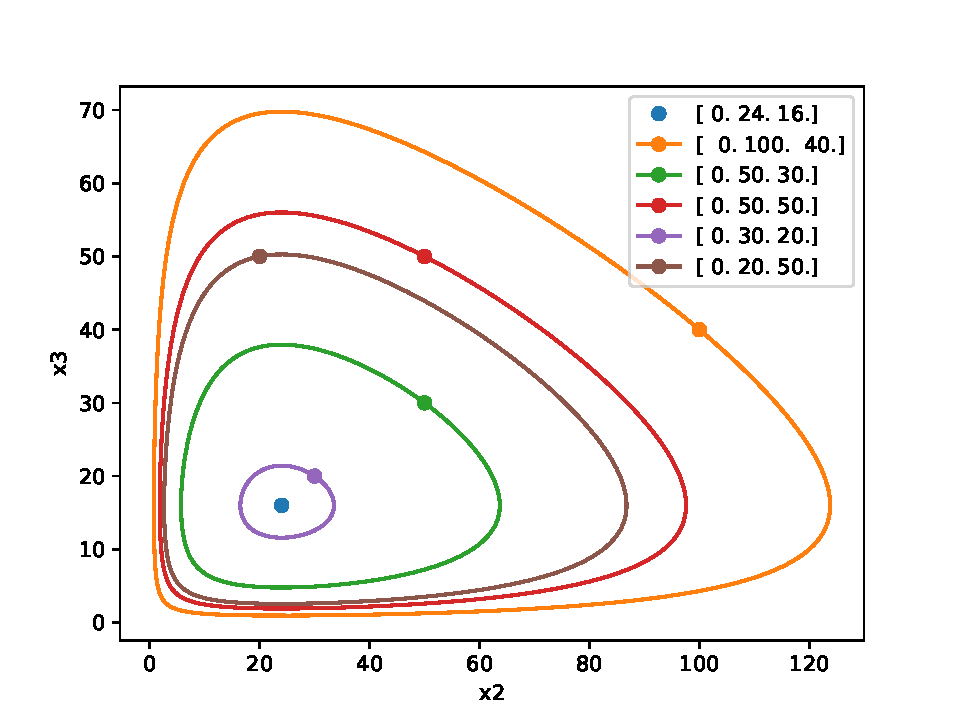
\includegraphics[width=8cm]{pictures/x1_0phase.pdf}
        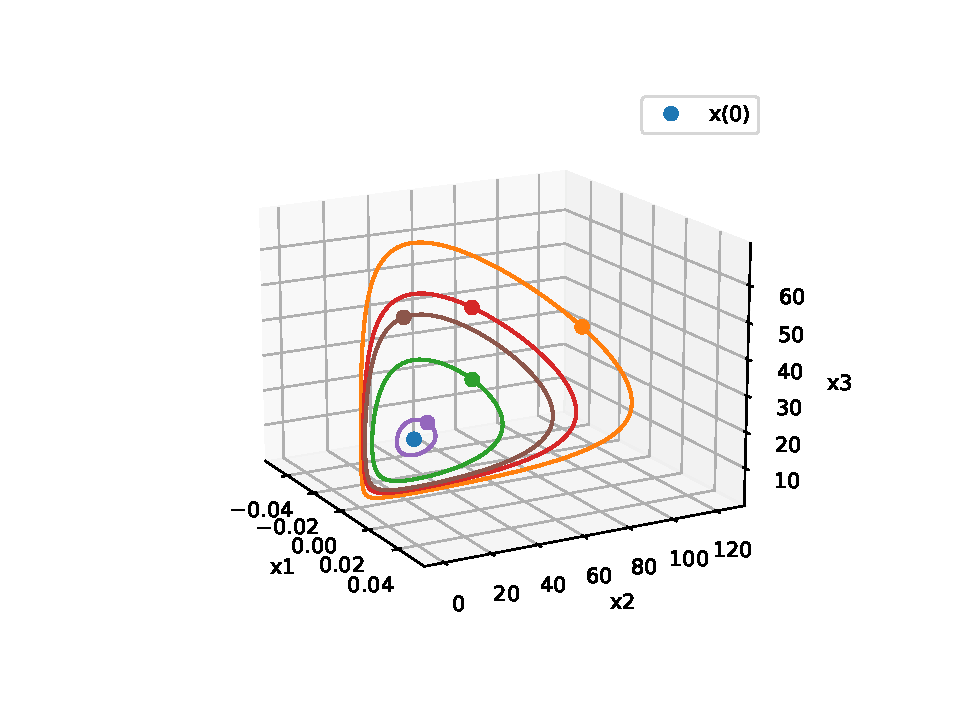
\includegraphics[width=8cm]{pictures/x1_0phase3.pdf}
        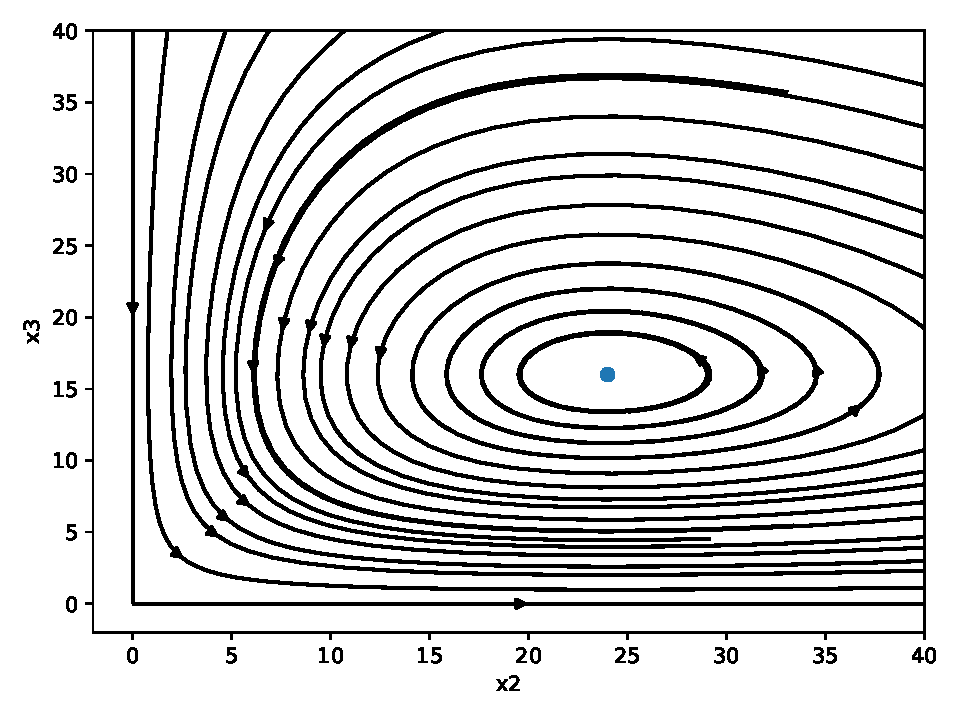
\includegraphics[width=8cm]{pictures/x1_0vector.pdf}
        \caption{На отрезке времени \( [0, 3] \).}
    \end{figure}


    \subsubsection{При вымершей второй популяции}

    \begin{figure}[H]
        \centering
        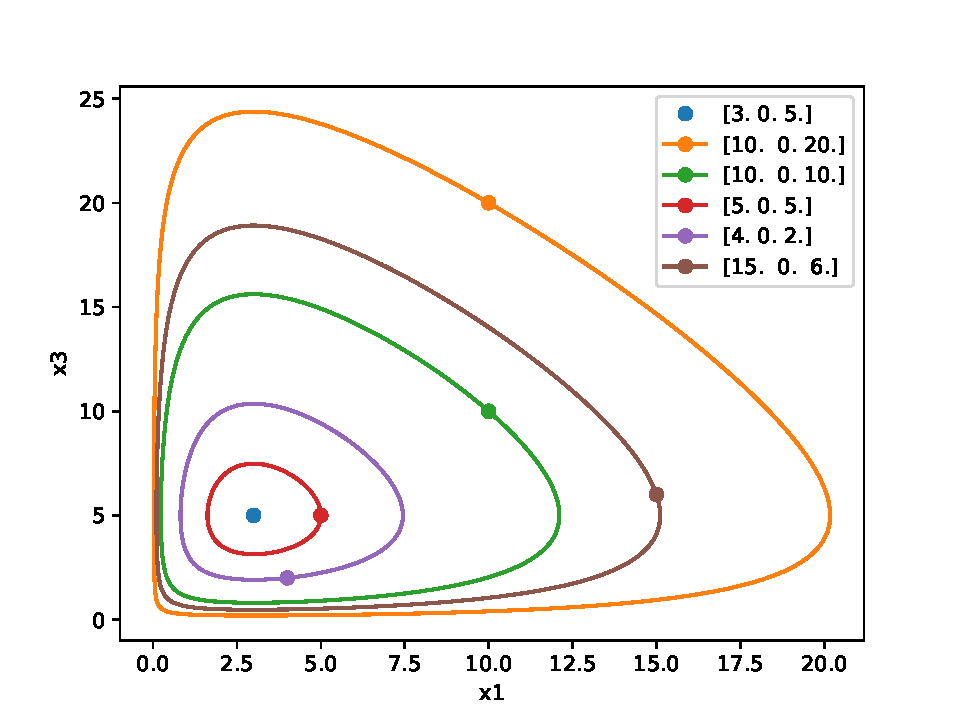
\includegraphics[width=8cm]{pictures/x2_0phase.pdf}
        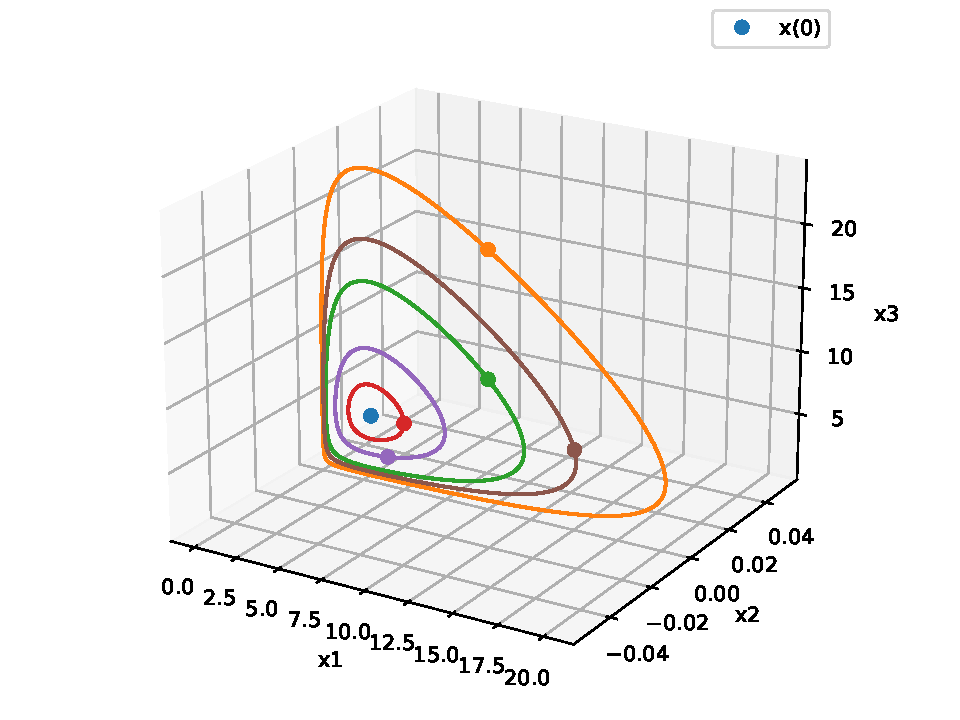
\includegraphics[width=8cm]{pictures/x2_0phase3.pdf}
        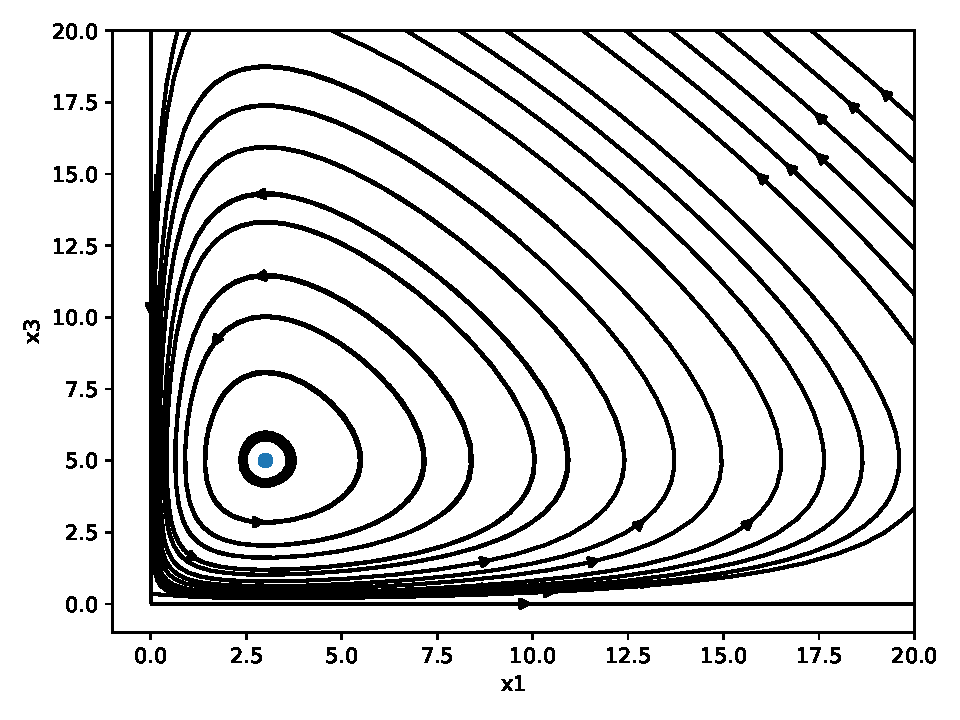
\includegraphics[width=8cm]{pictures/x2_0vector.pdf}
        \caption{На отрезке времени \( [0, 3] \).}
    \end{figure}


    \subsubsection{При вымершей третьей популяции}

    \begin{figure}[H]
        \centering
        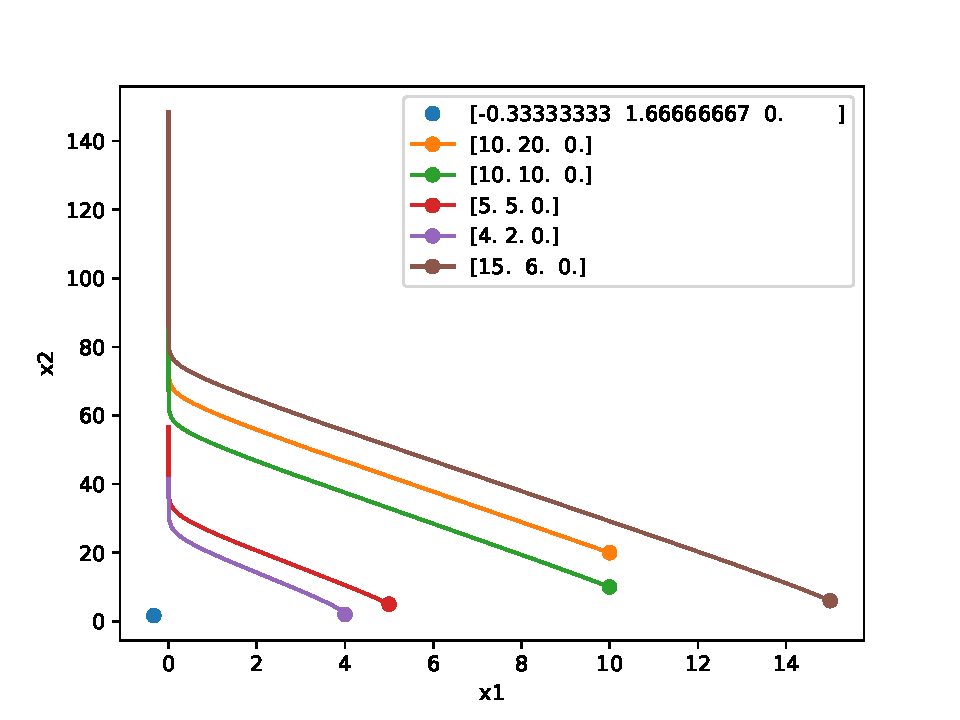
\includegraphics[width=8cm]{pictures/x3_0phase.pdf}
        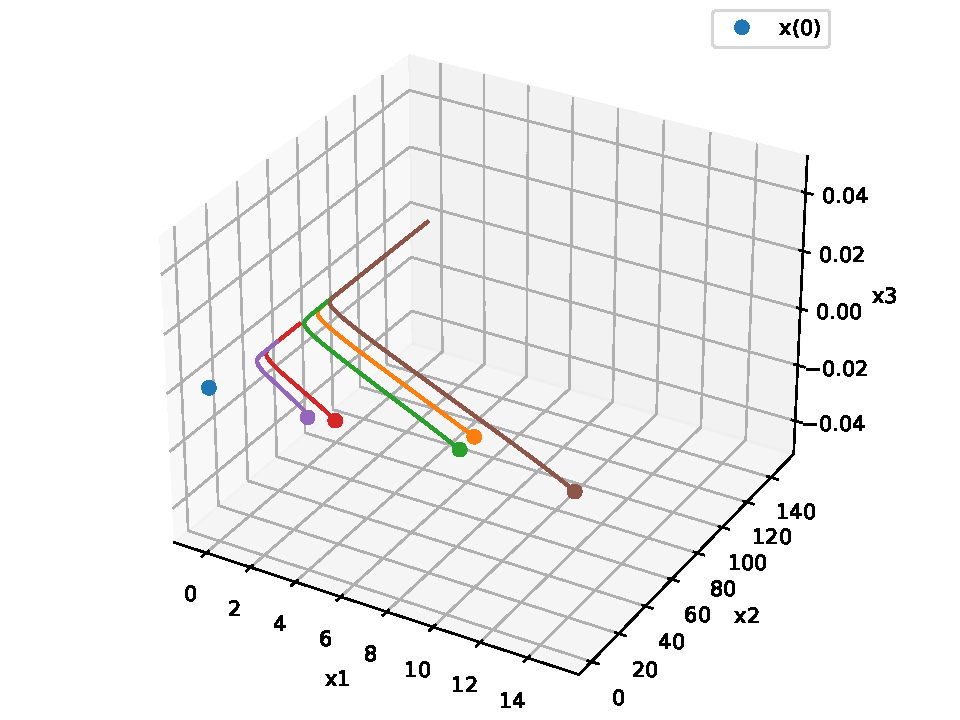
\includegraphics[width=8cm]{pictures/x3_0phase3.pdf}
        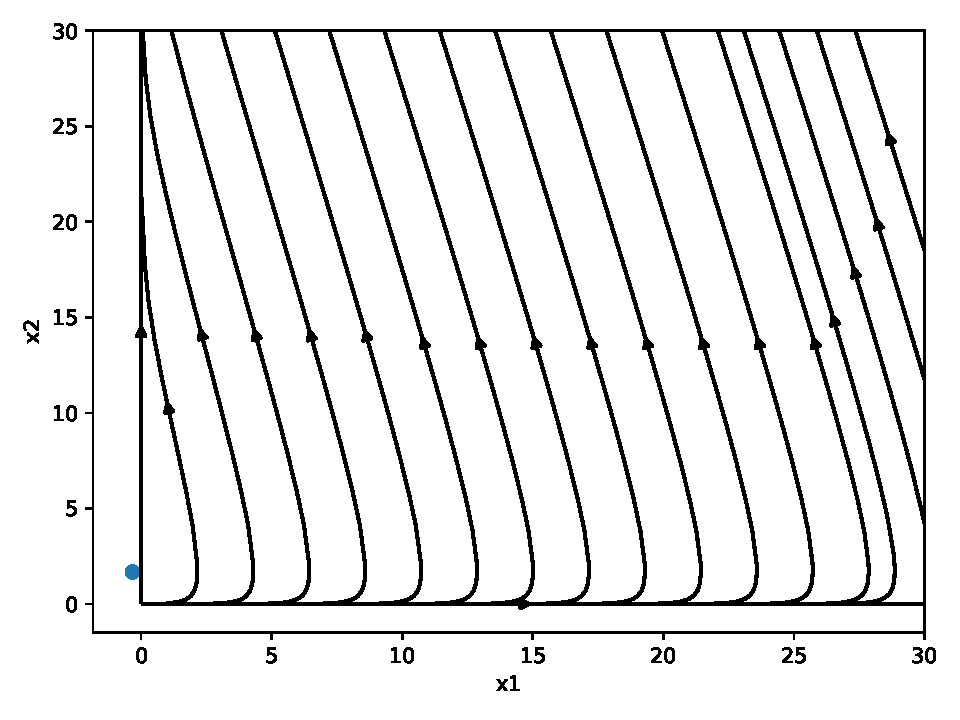
\includegraphics[width=8cm]{pictures/x3_0vector.pdf}
        \caption{На отрезке времени \( [0, 0.1] \).}
    \end{figure}

    \subsubsection{Несколько изначально не вымерших популяций}
    \begin{figure}[H]
        \centering
        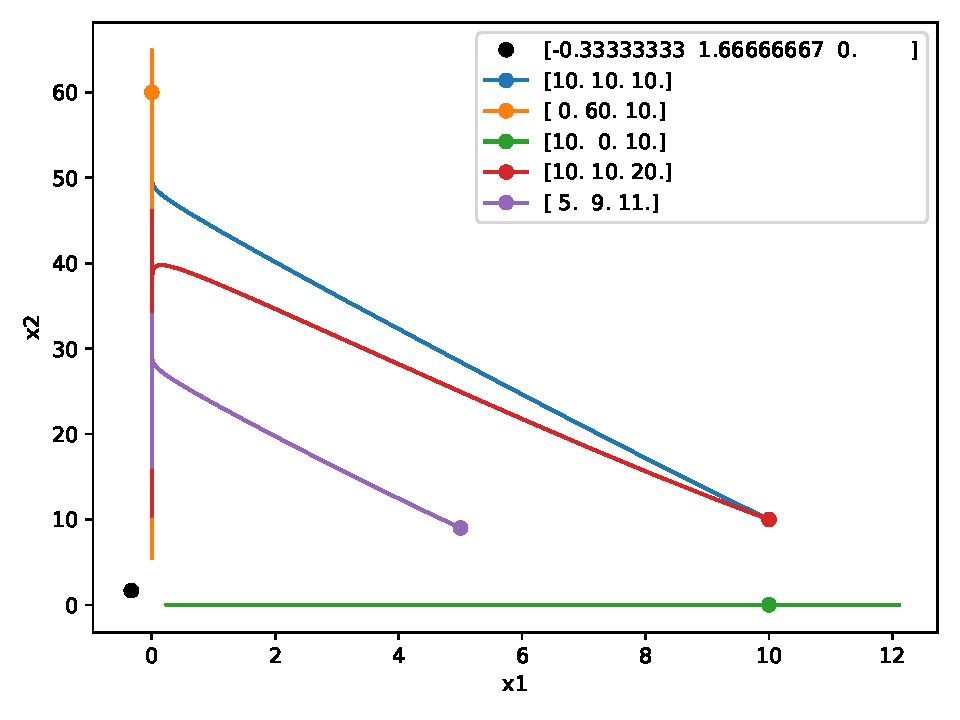
\includegraphics[width=8cm]{pictures/x_12phase.pdf}
        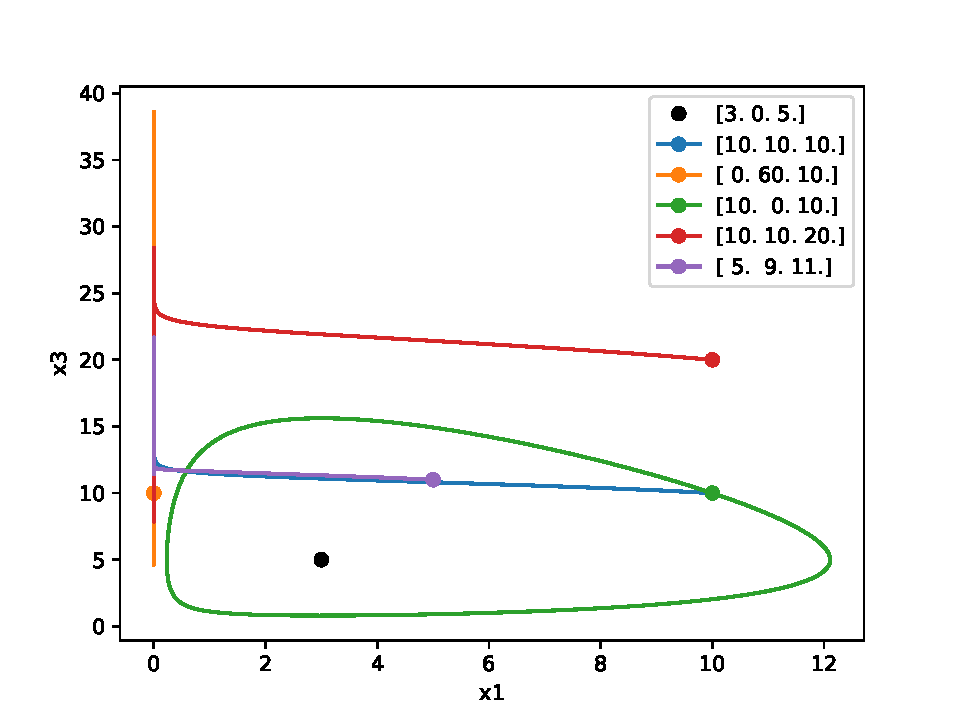
\includegraphics[width=8cm]{pictures/x_13phase.pdf}
        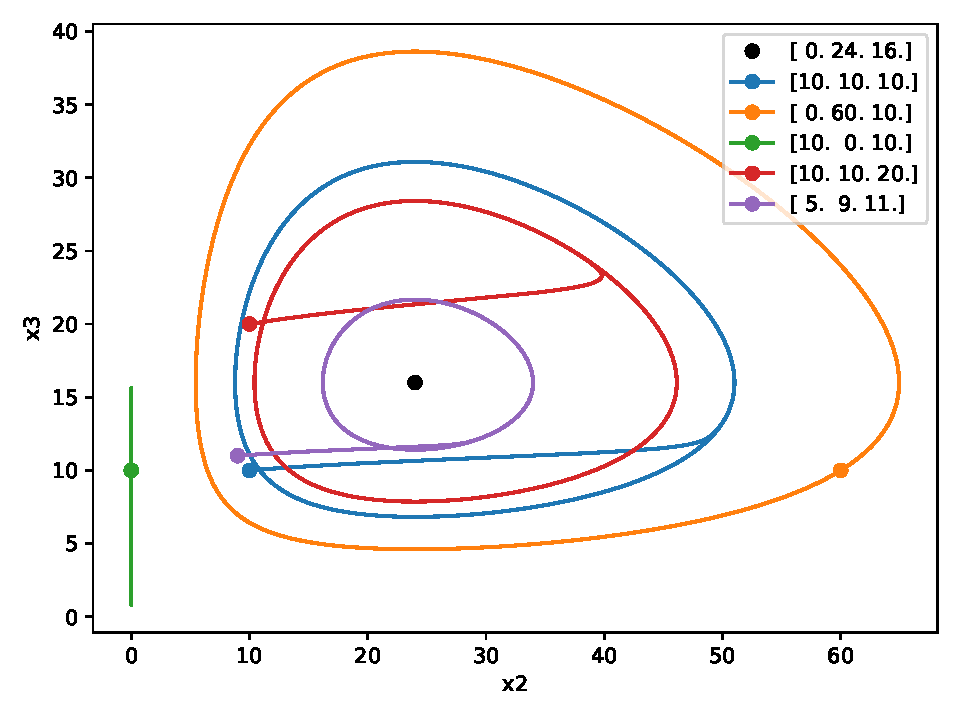
\includegraphics[width=8cm]{pictures/x_23phase.pdf}
        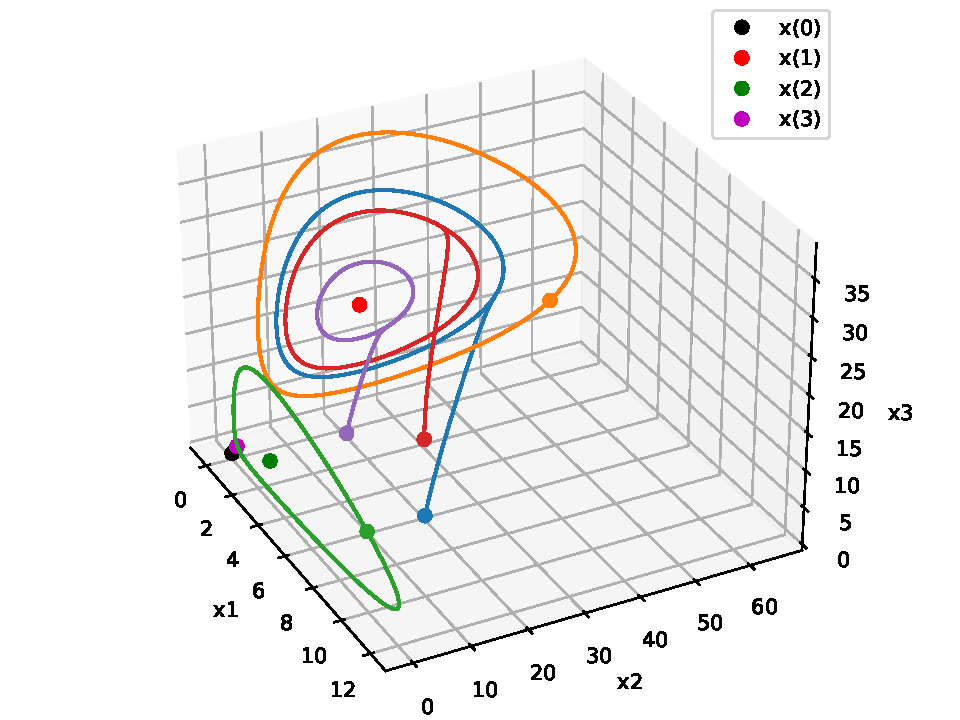
\includegraphics[width=8cm]{pictures/x_phase3.pdf}
        \caption{На отрезке времени \( [0, 3] \).}
    \end{figure}


    \pagebreak
    
    \section{Модель Колмогорова}

    \subsection{Математическая модель}
    Моделью Колмогорова при одной популяции жертвы \(x (t)\) и одной хищника \(y (t)\) называется такая модель \cite{svilog}:
    \[
        \left\{\begin{split}
            & \dot{x} = \alpha(x)x - V(x) y, \\
            & \dot{y} = K(x) y,
        \end{split}\right.
    \]
    с такими предположениями:
    
    \begin{enumerate}
        \item В популяции хищников отсутствует внутривидовая конкуренция.
        \item \( \alpha' < 0; ~ \alpha(0) > 0 > \alpha(\infty) \). В отсутствии хищников прирост жертв с увеличением популяции уменьшается до критического момента.
        \item \( K' > 0; ~ K(0) < 0 < K(\infty) \). Коэффициент прироста хищников.
        \item \( V(x) > 0, x > 0; ~ V(0) = 0 \). Коэффициент поглощения жертв.
    \end{enumerate}

    Адаптируем данную модель для нашей схемы взаимодеиствия популяций жертвы и хищников и подробнее опишем качественные предположения о функциях:
    \[
        \left\{\begin{split}
            & \dot{x_1} = \varepsilon(x_1)x_1 - V_{12}(x_1)x_2 - V_{13}(x_1)x_3, \\
            & \dot{x_2} = K_{12}(x_1)x_2 - V_{23}(x_2)x_3, \\
            & \dot{x_3} = K_{13}(x_1)x_3 + K_{23}(x_2)x_3. 
        \end{split}\right.
    \]
    Сформулируем предположения:
    \begin{enumerate}
        \item \( \varepsilon' < 0; ~ \varepsilon(0) > \varepsilon(\bar{x}_1) = 0 > \varepsilon(\infty)\). Здесь у жертв ограниченное количество ресурса и за него существует конкуренция. Поэтому без хищников прирост жертв с увеличением их количества в некоторый момент прекратится и стабилизируется на уровне \( \bar{x}_1 \).
        \item \( K'_{ij} > 0; ~ K_{ij}(0) < K_{ij}(x_i^*) = 0 < K_{ij} (\infty) \). Это значит, что при увеличении численности жертв коэффициент естественного прироста хищников возрастает. Коэффициент переходит от отрицательных значения при недостатке пищи к положительным.
        \item \( V_{ij}(0) = 0; ~ V_{ij} (x_i) > 0, x_i > 0 \). Этот коэффициент показывает количество жертв, поглощаемых одним хищником.
    \end{enumerate}

    Имеем автономную систему \( \dot{x} = f(x) \).

    Будем исследовать систему с линейными функциями, которые удовлетворяют указанным предположениям.
    \[
        \begin{split}
            & \varepsilon(x) = -\varepsilon \cdot x + \delta, & ~ \varepsilon, \delta > 0, \\
            & K_{ij} (x) = k_{ij} \cdot x - m_{ij}, & ~ k_{ij}, m_{ij} > 0, \\
            & V_{ij} (x) = v_{ij} \cdot x, & ~ v_{ij} > 0. 
        \end{split}
    \]

    Тогда система будет выглядеть так:
    \[
        \left\{\begin{split}
            & \dot{x_1} = \left( -\varepsilon x_1 + \delta \right)x_1 - v_{12} x_1 x_2 - v_{13} x_1 x_3, \\
            & \dot{x_2} = \left( k_{12} x_1 - m_{12} \right)x_2 - v_{23} x_2 x_3, \\
            & \dot{x_3} = \left( k_{13} x_1 - m_{13} \right)x_3 + \left( k_{23} x_2 - m_{23} \right)x_3. 
        \end{split}\right.
    \]

    \pagebreak

    \subsection{Анализ модели}
    Найдём точки равновесия дифференциального уравнения и исследуем их устойчивость.

    Матрица Якоби:
    \[
        J = \left(
            \begin{matrix}
                -2 \varepsilon x_1 + \delta - v_{12} x_2 - v_{13} x_3 & -v_{12}  x_1  & -v_{13} x_1 \\
                k_{12} x_2 & \left( k_{12} x_1 - m_{12} \right) - v_{23} x_3 & -v_{23} x_2 \\
                k_{13} x_3 & k_{23} x_3 & k_{13} x_1 - m_{13} + k_{23} x_2 - m_{23}
            \end{matrix}
        \right)
    \]

    Нужно найти решения \( (x_1, x_2, x_3) \) системы уравнений:
    \[
        \left\{\begin{split}
            & \left( -\varepsilon x_1 + \delta \right)x_1 - v_{12} x_1 x_2 - v_{13} x_1 x_3 = 0, \\
            & \left( k_{12} x_1 - m_{12} \right)x_2 - v_{23} x_2 x_3 = 0, \\
            & \left( k_{13} x_1 - m_{13} \right)x_3 + \left( k_{23} x_2 - m_{23} \right)x_3 = 0. 
        \end{split}\right.
    \]
    Для удобства вынесем общие множители:
    \[
        \left\{\begin{split}
            & \left( -\varepsilon x_1 + \delta - v_{12} x_2 - v_{13} x_3\right)x_1 = 0, \\
            & \left( k_{12} x_1 - m_{12} - v_{23} x_3 \right)x_2 = 0, \\
            & \left( k_{13} x_1 - m_{13} + k_{23} x_2 - m_{23} \right)x_3  = 0. 
        \end{split}\right.
    \]

    \begin{enumerate}
        \item Если \( x_2 = x_3 = 0 \), то остаётся уравнение 
        \[ ( -\varepsilon x_1 + \delta ) x_1 = 0. \] 
        Получаем тривиальное решение \( x^{(0)} = (0,0,0) \) и \( x^{(1)} = \left(\frac{\delta}{\varepsilon}, 0, 0 \right) \).
        \begin{enumerate}
            \item \( J \big|_{x^{(0)}} = \left(
                \begin{matrix}
                    \delta & 0 & 0 \\
                    0 & -m_{12}  & 0 \\
                    0 & 0 & -m_{23} (0)
                \end{matrix}
            \right) \)

            \[
                \lambda_1 = \delta> 0, ~
                \lambda_2 = -m_{12} < 0, ~
                \lambda_3 = -m_{23} < 0.
            \]

            Значит, в плоскостях \( x_2 = 0 \) и \( x_3 = 0 \) начало координат является седлом и направление \( x_1 \) -- неустойчивое. В плоскости \( x_1 = 0 \) точка является устойчивым узлом.

            \item \( J \big|_{x^{(1)}} = \left(
                \begin{matrix}
                    -\delta & -v_{12} \frac{\delta}{\varepsilon} & -v_{13} \frac{\delta}{\varepsilon} \\
                    0 & k_{12} \frac{\delta}{\varepsilon} - m_{12} & 0 \\
                    0 & 0 & k_{13} \frac{\delta}{\varepsilon} -m_{13} - m_{23}
                \end{matrix}
            \right) \)

            \[
                \lambda_1 = -\delta < 0, ~
                \lambda_2 = k_{12} \frac{\delta}{\varepsilon} - m_{12}, ~
                \lambda_3 = k_{13} \frac{\delta}{\varepsilon} -m_{13} - m_{23}. 
            \]
            Откуда имеем:
            \[
                \lambda_2 < 0 \Leftrightarrow \frac{\delta}{\varepsilon} < \frac{m_{12}}{k_{12}},
                \quad
                \lambda_3 < 0 \Leftrightarrow \frac{\delta}{\varepsilon} < \frac{m_{13} + m_{23}}{k_{13}}
            \]

            В зависимости от значений \( \lambda_2, \lambda_3 \) данная точка может быть:
            \begin{enumerate}
                \item Устойчивым узлом, если \( \lambda_2, \lambda_3 < 0 \),
                \item Устойчивым узлом в плоскости \( x_2 = 0 \) и седлом в плоскости \( x_3 = 0 \), если \( \lambda_2 > 0, \lambda_3 < 0 \),
                \item Устойчивым узлом в плоскости \( x_3 = 0 \) и седлом в плоскости \( x_2 = 0 \), если \( \lambda_2 < 0, \lambda_3 > 0 \),
                \item Седлом в плоскостях \( x_2 = 0, ~ x_3 = 0 \), если \( \lambda_2, \lambda_3 > 0 \)
            \end{enumerate}
            
            
        \end{enumerate}


        \item Если \( x_1 = x_2 = 0 \), то в третьей строчке получем
        \[ \left( -m_{13} -m_{23} \right) x_3 = 0. \]
        Поскольку \( x_3 > 0\), то данное равенство не может быть выполнено.


        \item Если \( x_1 = x_3 = 0 \), то во второй строчке получем
        \[ -m_{12} x_2 = 0. \]
        Поскольку \( x_2 > 0 \), то равенство не может быть выполнено.


        \item Если \( x_1 = 0; x_2, x_3 > 0 \):
            \[
                \left\{\begin{split}
                    & \left( -m_{12} - v_{23} x_3 \right) x_2 = 0, \\
                    & \left( -m_{13} + k_{23} x_2 - m_{23} \right) x_3 = 0. 
                \end{split}\right.
                \Rightarrow
                \left\{\begin{split}
                    & x_3 = \frac{ m_{12} }{ -v_{23} } < 0, \\
                    & x_2 = \frac{m_{13} + m_{23}}{k_{23}} . 
                \end{split}\right.
            \]
            Эта точка будет находиться вне исследуемой области.
        \item Если \( x_2 = 0; x_1, x_3 > 0 \):
            \[
                \left\{\begin{split}
                    & \left( -\varepsilon x_1 + \delta - v_{13} x_3 \right)x_1 = 0, \\
                    & \left( k_{13} x_1 -m_{13} - m_{23} \right)x_3 = 0. 
                \end{split}\right.
                \Rightarrow
                \left\{\begin{split}
                    & x_3 = \frac{ \varepsilon x_1 - \delta }{ -v_{13} }, \\
                    & x_1 = \frac{m_{13} + m_{23}}{k_{13}}. 
                \end{split}\right.
            \]
            В исследуемой области данная точка будет находиться, если \( x_1 \leq \frac{\delta}{\varepsilon} \).
            \[
                J \big|_{x^{(2)}} = \left(
                    \begin{matrix}
                        -\varepsilon x_1 & -v_{12}  x_1  & -v_{13} x_1 \\
                        0 & \left( k_{12} x_1 - m_{12} \right) - v_{23} x_3 & 0 \\
                        k_{13} x_3 & k_{23} x_3 & 0
                    \end{matrix}
                \right)
            \]
            FFF
            % \[
            %     \lambda_1 = \varepsilon \frac{m_{13} + m_{23}}{k_{13}} > 0, ~ 
            %     \lambda_2 = \left( k_{12} \frac{m_{13} + m_{23}}{k_{13}} - m_{12} \right) - v_{23} \frac{ \varepsilon x_1 - \delta }{ -v_{13} }, ~ 
            %     \lambda_3 = 0
            % \]

            % где-то будут линии FFF

        \item Если \( x_3 = 0; x_1, x_2 > 0 \):
            \[
                \left\{\begin{split}
                    & \left( -\varepsilon x_1 + \delta - v_{12} x_2 \right)x_1 = 0, \\
                    & ( k_{12} x_1 -m _{12} ) x_2 = 0. 
                \end{split}\right.
                \Rightarrow
                \left\{\begin{split}
                    & x_2 = \frac{ \varepsilon x_1 - \delta }{ -v_{12} }, \\
                    & x_1 = \frac{m_{12}}{k_{12}}. 
                \end{split}\right.
            \]
            В исследуемой области данная точка будет находиться, если \( x_1 \leq \frac{\delta}{\varepsilon}  \). FFF
            \[
                J\big|_{x^{(3)}} = \left(
                    \begin{matrix}
                        -\varepsilon x_1 & -v_{12}  x_1  & -v_{13} x_1 \\
                        k_{12} x_2 & 0 & -v_{23} x_2 \\
                        0 & 0 & k_{13} x_1 - m_{13} + k_{23} x_2 - m_{23}
                    \end{matrix}
                \right)
            \]
        \item Если \( x_1, x_2, x_3 > 0 \):
            \[
                \left\{\begin{split}
                    & -\varepsilon x_1 + \delta - v_{12} x_2 - v_{13} x_3 = 0, \\
                    & k_{12} x_1 - m_{12} - v_{23} x_3 = 0, \\
                    & k_{13} x_1 - m_{13} + k_{23} x_2 - m_{23} = 0. 
                \end{split}\right.
            \]

            \[
                \left\{\begin{split}
                    & x_1 = \frac{-\delta k_{23} v_{23} - k_{23} m_{12} v_{13} + m_{13} v_{12} v_{23} + m_{23} v_{12} v_{23}}{-\varepsilon k_{23} v_{23} - k_{12} k_{23} v_{13} + k_{13} v_{12} v_{23}}, \\
                    & x_2 = \frac{\delta k_{13} v_{23} - \varepsilon m_{13} v_{23} - \varepsilon m_{23} v_{23} - k_{12} m_{13} v_{13} - k_{12} m_{23} v_{13} + k_{13} m_{12} v_{13}}{-\varepsilon k_{23} v_{23} - k_{12} k_{23} v_{13} + k_{13} v_{12} v_{23}}, \\
                    & x_3 = \frac{-\delta k_{12} k_{23} + \varepsilon k_{23} m_{12} + k_{12} m_{13} v_{12} + k_{12} m_{23} v_{12} - k_{13} m_{12} v_{12}}{-\varepsilon k_{23} v_{23} - k_{12} k_{23} v_{13} + k_{13} v_{12} v_{23}}
                \end{split}\right.
            \]

            \[
                J = \left(
                    \begin{matrix}
                        -2 \varepsilon x_1 + \delta - v_{12} x_2 - v_{13} x_3 & -v_{12}  x_1  & -v_{13} x_1 \\
                        k_{12} x_2 & \left( k_{12} x_1 - m_{12} \right) - v_{23} x_3 & -v_{23} x_2 \\
                        k_{13} x_3 & k_{23} x_3 & k_{13} x_1 - m_{13} + k_{23} x_2 - m_{23}
                    \end{matrix}
                \right)
            \]


    \end{enumerate}

    \pagebreak

    \subsection{Вычислительные эксперименты}
    Возьмём такие функции для построения модели:
    \[
        \begin{split}
            & \varepsilon (x_1) = -x_1 + 10, \\
            & K_{12} (x_1) = x_1 - 5, ~ K_{13} (x_1) = x_1 - 3, ~ K_{23} (x_2) = x_2 - 4, \\
            & V_{12} (x_1) = 2 x_1, ~ V_{13} (x_1) = 3 x_1, ~ V_{23} (x_2) = x_2.
        \end{split}
    \]

    \subsubsection{При вымершей первой популяции}

    \begin{figure}[H]
        \centering
        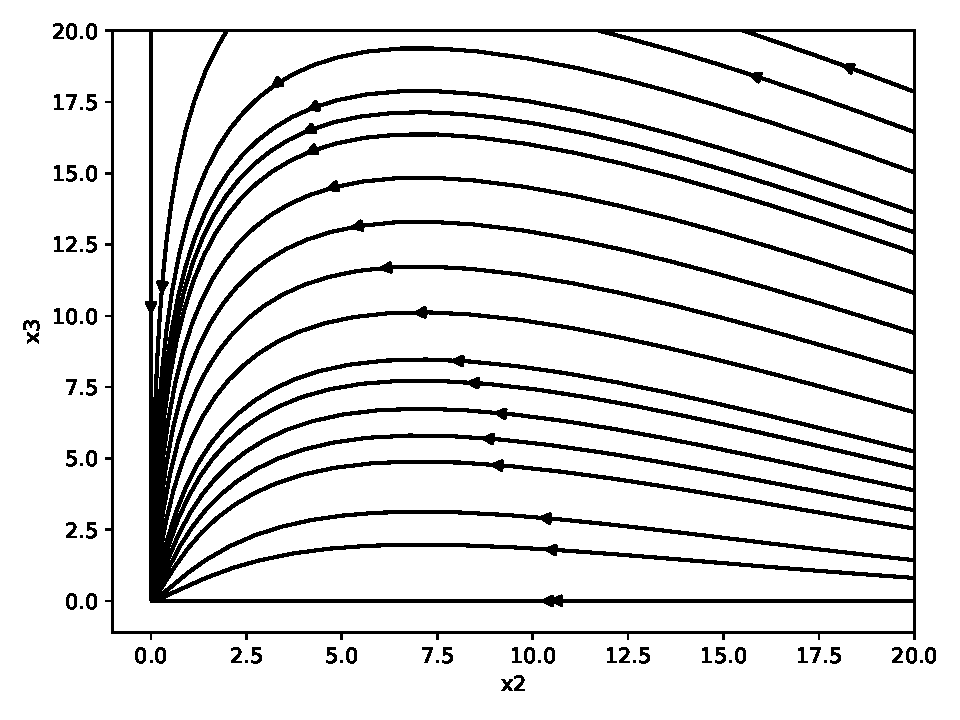
\includegraphics[width=8cm]{pictures/kx1_0vector.pdf}
    \end{figure}


    \subsubsection{При вымершей второй популяции}

    \begin{figure}[H]
        \centering
        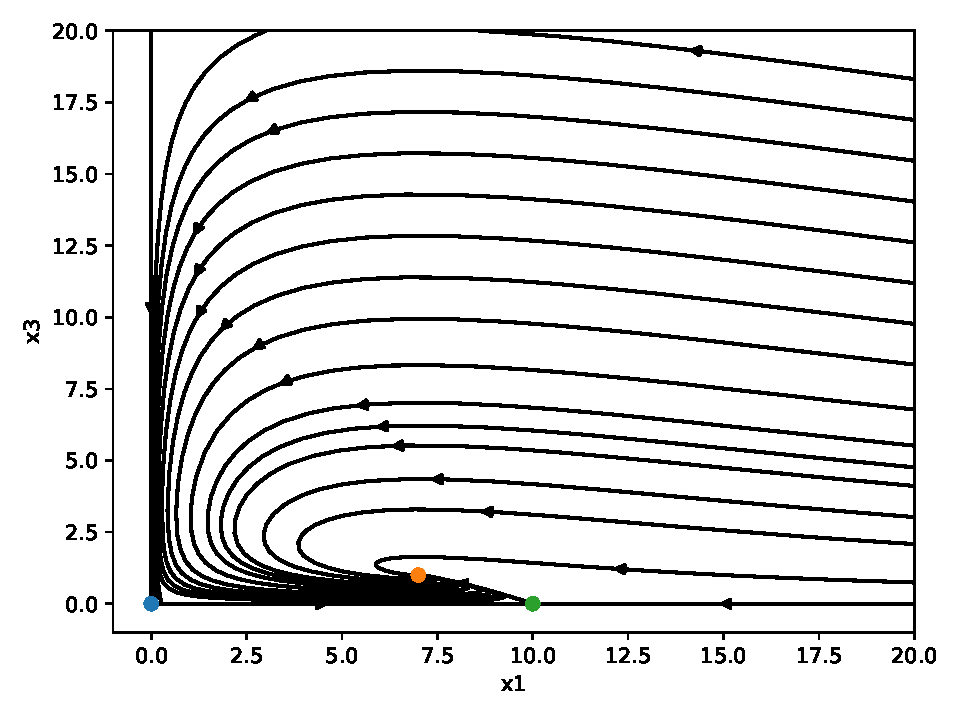
\includegraphics[width=8cm]{pictures/kx2_0vector.pdf}
    \end{figure}


    \subsubsection{При вымершей третьей популяции}

    \begin{figure}[H]
        \centering
        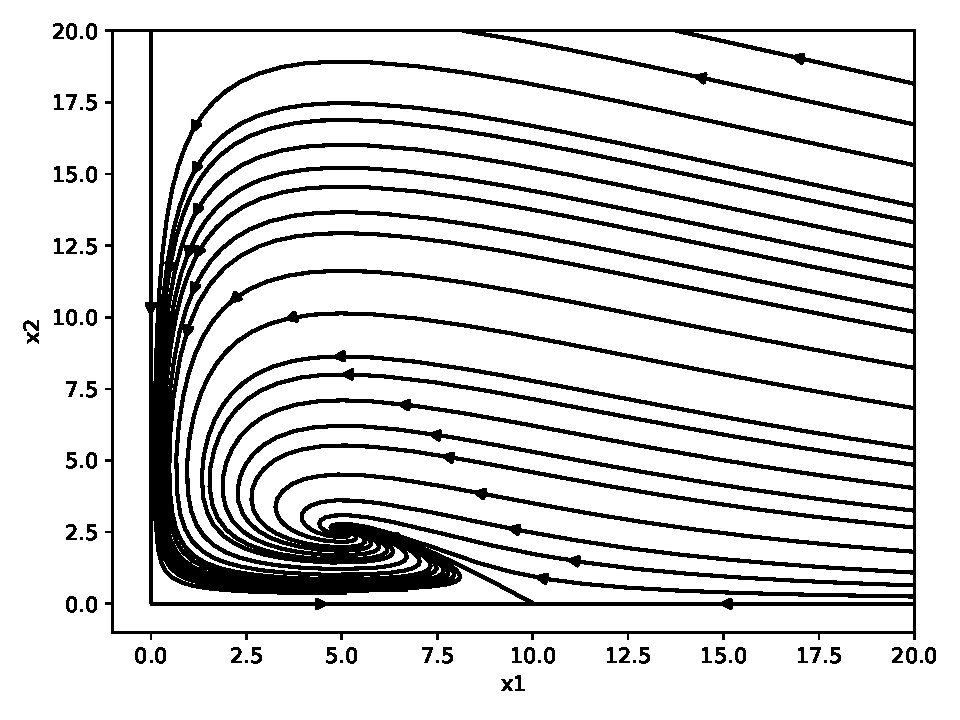
\includegraphics[width=8cm]{pictures/kx3_0vector.pdf}
    \end{figure}

    \subsubsection{Несколько изначально не вымерших популяций}
    \begin{figure}[H]
        \centering
        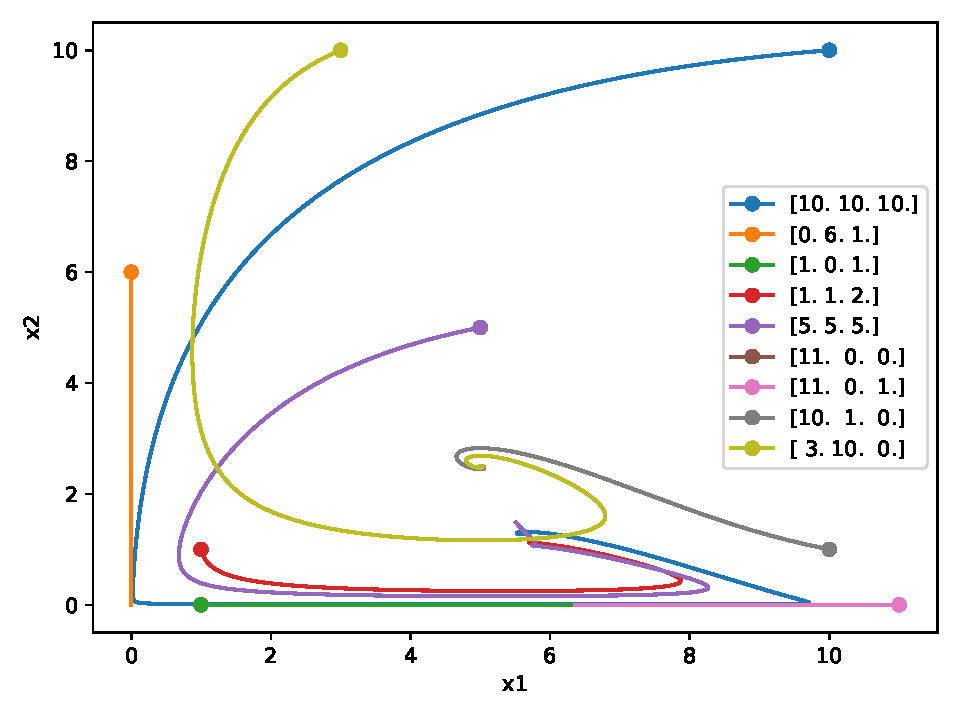
\includegraphics[width=8cm]{pictures/kx_12phase.pdf}
        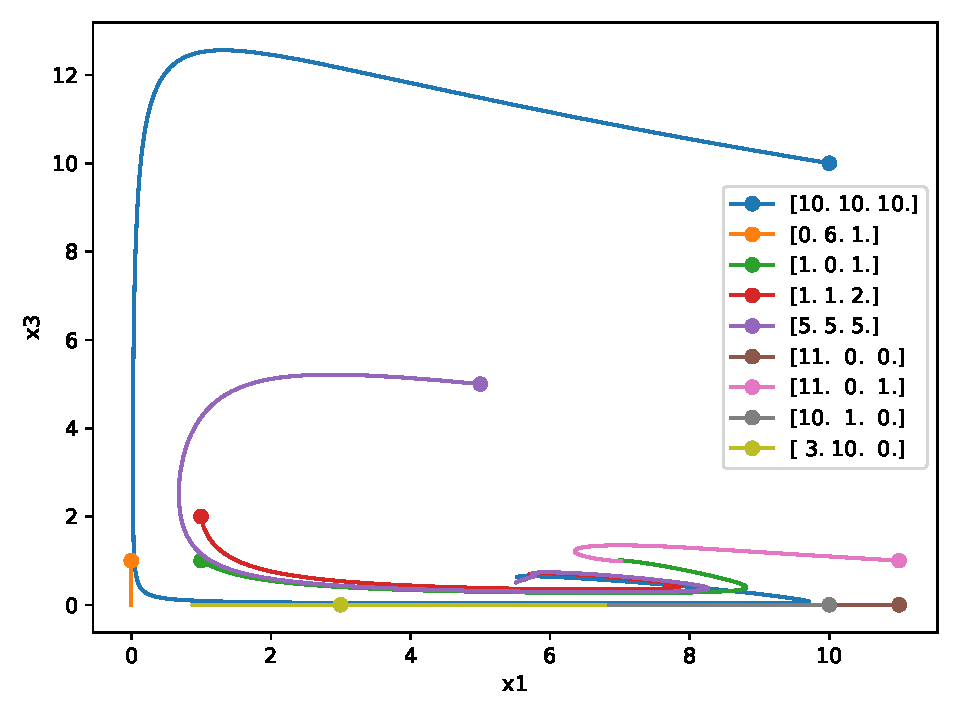
\includegraphics[width=8cm]{pictures/kx_13phase.pdf}
        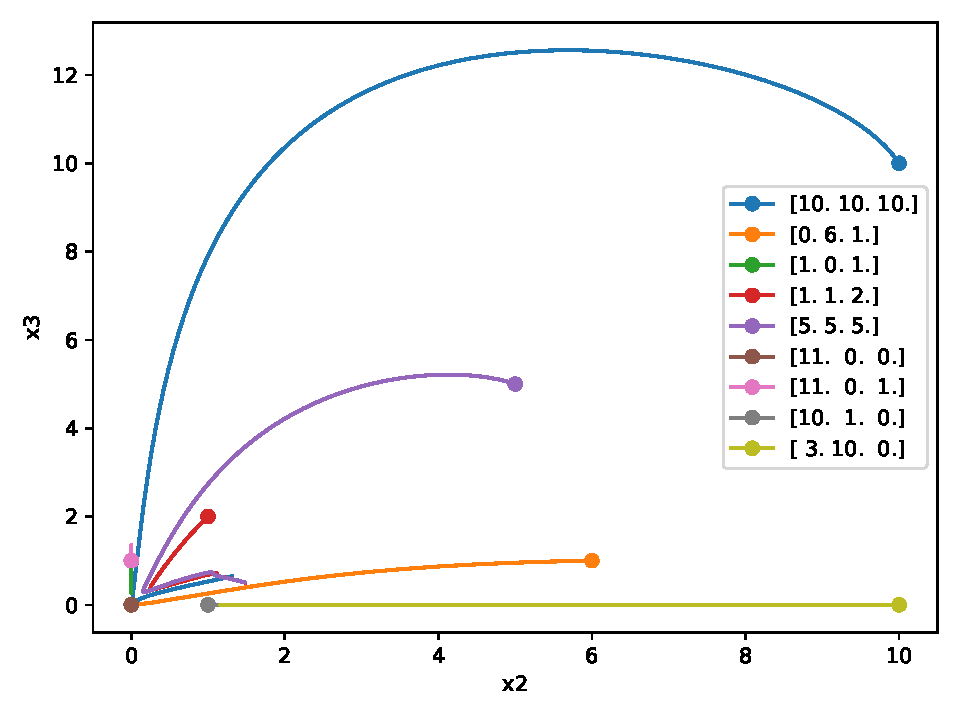
\includegraphics[width=8cm]{pictures/kx_23phase.pdf}
        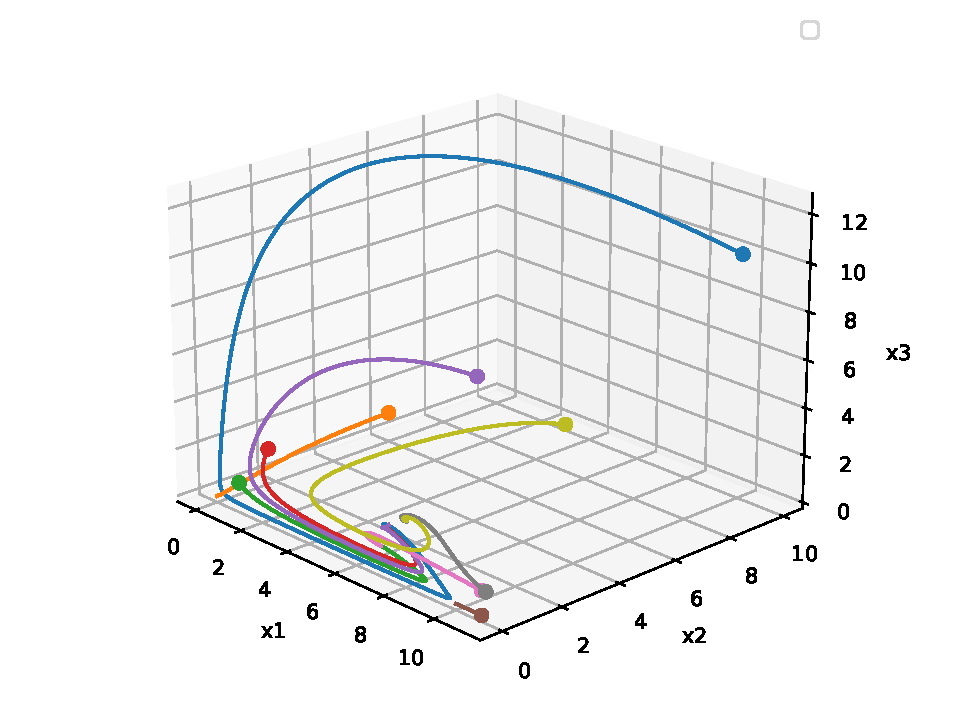
\includegraphics[width=8cm]{pictures/kx_phase3.pdf}
        \caption{На отрезке времени \( [0, 3] \).}
    \end{figure}

    \pagebreak

    \section{Заключение}
    Таким образом, была построена математическая модель электрического нагревателя с терморегулятором и без него. Модель представляет из себя дифференциальное уравнение. Данная модель была проанализирована и были найдены точки равновесия дифференциального уравнения. Написана программа для численного решения решения уравнения в зависимости от параметров. Проведены вычислительные эксперименты, которые соответствуют с результатам анализа.

    \pagebreak

    \begin{thebibliography}{9}
    \bibitem{svilog}
        Свирежев, Ю. М. Устойчивость биологических сообществ // Ю. М. Свирежев, Д. О. Логофет -- М.: Наука, 1978.

    \bibitem{pont}
        Понтрягин, Л. С. Обыкновенные дифференциальные уравнения // Л. С. Понтрягин -- М.: Наука, 1974.

    \bibitem{filipov}
        Филипов, А. Ф. Введение в теорию дифференциальных уравнений // А. Ф. Филипов -- М.: КомКнига, 2007.
    
    \bibitem{nefedov}
        Нефёдов, Н. Н. Обыкновенные дифференциальные уравнения // Н. Н. Нефёдов, В. Ю. Попов, В. Т. Волков -- М.: Физический факультет МГУ им. М. В. Ломоносова, 2016.

    \bibitem{berez}
        Березин, И. С. Методы вычислений // И. С. Березин, Н. П. Жидков -- М.: Наука, 1959. -- Т. 2.

\end{thebibliography}

\end{document}